% !TEX root =  ../report.tex
\section{Introduction}
First things first, we started this project with a {\color{blue}\href{https://www.kaggle.com/code/luiscruz/phishing-detection-cnn?scriptVersionId=173193829}{Machine Learning model}} for detecting URL phishing, which is the act of fraudulently manipulating victims to click on links in order to obtain their credentials, banking information, or passwords. Our goal is to design an application around this model and deploy it, such that the application is production-ready. 
Therefore, in this document you will be able to find the overall setup of the project, with the corresponding design decisions we took in order to realize our goal. A link to our GitHub organization can be found here:
{\color{blue} \url{https://github.com/remla24-team12}}.

\subsection{Use Cases}
The use cases of the application are fairly straightforward: \\
Firstly, the user can provide a URL of their choice as input, then the model makes a prediction whether the URL is valid or phishing, finally the prediction is displayed to the user. \\
Afterwards, the user is asked to give feedback on the prediction. This will help improve the accuracy of the model over time: If the users deems the prediction to be incorrect, we can either update the label for the URL, or when the URL is not yet present in the dataset, we obtain a new entry with a human-verified label. 

\subsection{Architecture}
When designing the application we decided to stick to the architecture proposed in the assignment, see fig. {\color{red}\ref{fig:architecture}}.
For this micro-services architecture all components are built independently and interact with each other through package dependencies or APIs. \\
Every component is developed its own corresponding repository (except \texttt{app-frontend} and \texttt{app-service}, which are combined into one). Additionally, we use a \texttt{provisioning} repository which acts as the central repository containing all information about running the application and operating the cluster.
Regarding the purpose of the other components, we have the app:
\begin{itemize}
    \item \texttt{app-frontend} : Receives input from the user and forwards this to the \texttt{app-service} using an API.
    \item \texttt{app-service} : Middle man between frontend and backend, queries the \texttt{model-service} using an API and forwards this to the frontend.
    \item \texttt{lib-version} : Library containing version of the app, used for automatic versioning.
\end{itemize}

And the model:
\begin{itemize}
    \item \texttt{model-training} : Trains the model and stores it publicly such that the \texttt{model-service} can access it.
    \item \texttt{model-service} : Acts as a wrapper for the released model through an API. Receives request from \texttt{app-service}, queries the model and sends the response back.
    \item \texttt{lib-ml} : Contains pre-processing logic for data that is used for training or queries.
\end{itemize}

\begin{figure*}
    \centering
    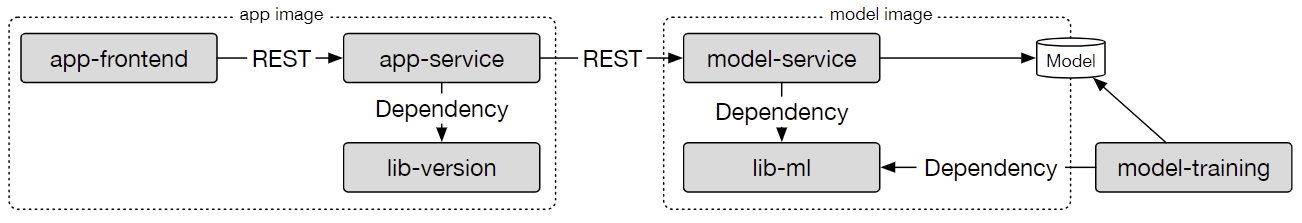
\includegraphics[width=1\linewidth]{images/architecture.png}
    \caption{Application Architecture}
    \label{fig:architecture}
\end{figure*}

